%% -----------------------------------------------------------------
%% This file uses UTF-8 encoding
%%
%% For compilation use following command:
%% latexmk -pdf -pvc -bibtex thesis
%%
%% -----------------------------------------------------------------
%%                                     _     _      
%%      _ __  _ __ ___  __ _ _ __ ___ | |__ | | ___ 
%%     | '_ \| '__/ _ \/ _` | '_ ` _ \| '_ \| |/ _ \
%%     | |_) | | |  __/ (_| | | | | | | |_) | |  __/
%%     | .__/|_|  \___|\__,_|_| |_| |_|_.__/|_|\___|
%%     |_|                                          
%%
%% -----------------------------------------------------------------

\documentclass{kithesis}

% Additional packages
\usepackage[main=slovak,english]{babel}
% For thesis written in English just change the order of languages:
% \usepackage[main=english,slovak]{babel}

\usepackage{listings}  % for source code
% Listings settings
% See for details: https://en.wikibooks.org/wiki/LaTeX/Source_Code_Listings
\lstset{
    basicstyle=\small\ttfamily,  % smaller typewriter font
    showstringspaces=false       % don't show spaces in string
}

% Location of file with bibliography resources
\addbibresource{chapters/bibliography.bib}

% Variables
%\thesisspec{figures/thesisspec.png} 

\title{My thesis \br (the skeleton)}{Moja záverečná práca \br (šablóna)}

%\author{Janko Hraško}
\author[Bc.]{Janko}{Hraško}[PhD.]
\supervisor{Leslie Lamport} %veduci prace
\consultant{Donald E. Knuth} %konzultant
%\college{University of Žilina}{Žilinská univerzita} %univerzita
%\faculty{Faculty of Electrical Engineering and informatics}{Fakulta elektrotechniky a informatiky} %fakulta
%\department{Department of Computers and Informatics}{Katedra počítačov a informatiky} %katedra
%\departmentacr{DCI}{KPI} % skratka katedry
%\thesis{Master thesis}{Diplomová práca} %typ prace
\submissiondate{13}{5}{2018}
%\fieldofstudy{9.2.1 Informatika}
%\studyprogramme{Informatika}
%\city{Košice} %mesto
\keywords{\LaTeX, programming, typesetting}{\LaTeX, programovanie, sadzba textu}
%\declaration{som nepodvadzal}

\abstract{%
    % english 
	\blindtext
}{%
    % slovak 
	\blindtext
}

\acknowledgment{Na tomto mieste by som rád poďakoval svojmu vedúcemu práce za jeho čas a odborné vedenie počas riešenia mojej záverečnej práce.

Rovnako by som sa rád poďakoval svojim rodičom a priateľom za ich podporu a povzbudzovanie počas celého môjho štúdia.
    
V neposlednom rade by som sa rád poďakoval pánom \textit{Donaldovi E. Knuthovi} a \textit{Leslie Lamportovi} za typografický systém \LaTeX, s ktorým som strávil množstvo nezabudnuteľných večerov.}

% if you want to work only on selected chapters
%\includeonly{chapters/analyza} %,chapters/synteza}

% Load acronyms
\input{acronyms}


%% -----------------------------------------------------------------
%%          _                                       _   
%%       __| | ___   ___ _   _ _ __ ___   ___ _ __ | |_ 
%%      / _` |/ _ \ / __| | | | '_ ` _ \ / _ \ '_ \| __|
%%     | (_| | (_) | (__| |_| | | | | | |  __/ | | | |_ 
%%      \__,_|\___/ \___|\__,_|_| |_| |_|\___|_| |_|\__|
%%                                                      
%% -----------------------------------------------------------------

\begin{document}
%% Title page, abstract, declaration etc.:
\frontmatter{}

%% List of code listings, if you are using package minted
%\listoflistings

%\pagenumbering{arabic}

%% Chapters
% !TEX root = ../thesis.tex

\chaptermark{Úvod}
\phantomsection
\addcontentsline{toc}{chapter}{Úvod}

\chapter*{Úvod}

Úvod práce stručne opisuje stanovený problém, kontext problému a motiváciu pre riešenie problému. Z~úvodu by malo byť jasné, že stanovený problém doposiaľ nie je vyriešený a má zmysel ho riešiť.
V~úvode neuvádzajte štruktúru práce, t.j. o~čom je ktorá kapitola. Rozsah úvodu je minimálne 2 celé strany (vrátane formulácie úlohy). Toto je skuska.

Ďalšie užitočné informácie môžete nájsť v~Pokynoch pre vypracovanie záverečných prác\footnote{\url{https://moodle.fei.tuke.sk/pluginfile.php/27971/mod_resource/content/16/Instructions_v15.pdf}}.


\section*{Formulácia úlohy}

Text záverečnej práce musí obsahovať sekciu s~formuláciou úlohy resp. úloh riešených v~rámci záverečnej práce. V~tejto časti autor rozvedie spôsob, akým budú riešené úlohy a~tézy formulované v~zadaní práce. Taktiež uvedie prehľad podmienok riešenia.

% !TEX root = ../thesis.tex

\chapter{Strojové učenie}

\section{Formy strojového učenia a typy dát}
Strojové učnie možeme rozdeliť na tri časti: učenie s učiteľom, učenie bez učiteľa a učenie posilňovaním.

Učenie s učiteľom je forma strojového učenia, pri ktorom majú naše dáta aj určené do ktorej triedy, ktorú chceme predikovať patria. Naše namerané X hodnoty najú svoje y.

Učenie bez učiteľa je prípad kedy naše dáta nemajú určenú triedu, ktorú potrebujeme predikovať. Algoritmus musí najsť triedy sám.

V prípade učnia s posilňovaním je učenie vykonávané formou spätnej väzby, kde v prípade správnej predikcie je algoritmus odmenený a v prípade nesprávnej potrestaný. 

Pre každú formu strojového učenia potrebujeme nejaké dáta, na ktorých sa bude náš model učiť a testovať. Dáta možu byť rôznych formátov ale najčastejšie ide o tabuľy pozostávajúce z uskutočnených meraní - vzoriek. Každá vzorka má svoje atribúty a v prípade učenia s učiteľom aj svoju triedu. 

\subsection{Proces strojového učenia}
Proces strojového učenia pozostáva z viacero časti. Prvou časťou je zber dát. V praxi častokrát dostane Machine learning engineer už pripravené dáta, ak firma zbierala dáta od zákazníkov alebo dostala výsledky prieskumu. Poprípade si vieme dáta zozbierať aj sami, napríklad vytvorením web scrappera, ktorý nám zozbiera dáta z webu.

Ďalšou časťou procesu je predspracovanie dát. Zo zozbieraných dát musíme vybrať dáta ktoré sú pre nás relevantné. Musíme sa usistiť že nemáme nejaké prázdne hodnoty, v takom prípade musíme buď zmazať celé jedno merianie, alebo tam imputovať priemerné hodnoty, Musíme premeniť znakové hodnoty na číselné, pričom musíme zohľadniť rozdiely medzi ordinálnymi a nominálnymi atribútmi. Ak máme veľký nepomer vo veľkosti číselných atribúov, musíme aplikovať škálovanie a/alebo normalizáciu. A v neposlednom rade musíme rozdeliť naše dáta na trénovacie a testovacie. Nesmie nastať situácia aby sme použili časť testovacích dát na trénovanie a naopak.

Keď máme spravené predspracovanie dát, môžeme sa pustiť do výberu modelu. Je ideálne si vyskúšať viacero možných algoritmov a zároveň aj parametrov. Pomocou cross-validácie zitíme ktorý model a jeho nastavenia budú najviac vyhovovať nášmu riešeniu. 

Keď máme náš model natrénvaný, môžeme pristúpiť k ďalšiemu kroku, čo je evaluácia modelu. Necháme zbehnuť náš model na testovacích dátach a necháme ho predikovať hodnoty. 

Ako posledná časť procesu je nasadenie modelu (deploy) do aplikácie. Táto časť procesu nie je súčasťou zadania, avšak ak by sme robili model do praxe, tak by sme napríklad chceli náš model na predikciu kníh, ktoré by sa mohli zákazníkovi páčiť, nasadiť do aplikácie knihkupectva.

\begin{figure}[!ht]
  \centering
  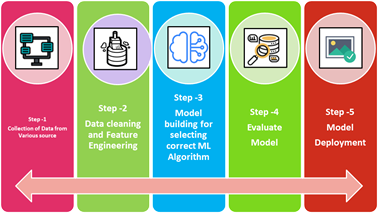
\includegraphics[width=1\textwidth]{figures/process.png}
  \caption{Proces strojové učenia}
  \cite{process}
\end{figure}

\subsection{sickitLarn}


\section{Porovnania cien nehnutelnosti}

\subsection{Lineárna regresia}

% !TEX root = ../thesis.tex

\chapter{Syntetická časť}
\label{methodology}

Syntetická časť opisuje metódy použité na syntézu riešenia a opisuje syntézu samotného riešenia (zvyčajne je to návrh/implementácia softvérového resp. hardvérového riešenia), pričom sa opiera o~závery analytickej časti práce. Začína od toho, ako sa bude riešenie používať: najdôležitejšie scenáre používania a používateľské rozhranie, ktoré bude tieto scenáre efektívne podporovať. Až potom je na rade vnútorná architektúra alebo použité technológie. Syntetická časť tvorí zvyčajne ½ jadra práce.

Syntetickú časť práce vhodne rozdeľte do kapitol a pomenujte ich podľa toho, čomu sú venované.

\begin{itemize}
  \item v~knihe \cite{book} autor prezentuje naozaj odvážne myšlienky
  \item nemenej zaujímavé výsledky publikuje ďalší autor v~článku \cite{article} 
  \item v~konferenčnom príspevku \cite{conference} sú uvedené tiež zaujímavé veci
  \item \LaTeX{}\footnote{\url{https://www.latex-project.org/}} je typografický jazyk
\end{itemize}



\begin{lstlisting}[language=C,caption={Program, ktorý pozdraví celý svet}]
  #include <stdio.h>
  int main() {
      /* Print Hello, World! */
      printf("Hello, World!\n");
      return 0;
  }
  \end{lstlisting}


  
\begin{table}[!ht]
	\caption{Country list}\label{t:1}
	\smallskip
	\centering

	\begin{tabular}{ |p{3cm}||p{3cm}|p{3cm}|p{3cm}|  }
		\hline
		\multicolumn{4}{|c|}{Country List} \\
		\hline
		Country Name or Area Name& ISO ALPHA 2 Code &ISO ALPHA 3 Code&ISO numeric Code\\
		\hline
		Afghanistan & AF & AFG & 004\\
		Aland Islands & AX & ALA & 248\\
		Albania & AL & ALB & 008\\
		Algeria & DZ & DZA & 012\\
		American Samoa & AS & ASM & 016\\
		Andorra & AD & AND & 020\\
		Angola & AO & AGO & 024\\
		\hline
	\end{tabular}
\end{table}

\include{chapters/evaluation}
\include{chapters/summary}

% good linebraking of bibtex url
\setcounter{biburllcpenalty}{7000}
\setcounter{biburlucpenalty}{8000}

%% The bibliography
\printbibliography[heading=bibintoc]

\label{theend} % the last page of the thesis

% List of acronyms
\printglossary[type=\acronymtype,title={\acrlistname}]

% Glossaries
\printglossary

%% Appendix
\include{appendixes/list}
\appendix
\renewcommand\chaptername{\appendixname}
\include{appendixes/prilohaa}

% zivotopis autora
%\curriculumvitae\protect
%Táto časť\/ je nepovinná. Autor tu môže uviesť\/ svoje biografické
%údaje, údaje o~záujmoch, účasti na~projektoch, účasti na~súťažiach,
%získané ocenenia, zahraničné pobyty na~praxi, domácu prax, publikácie
%a~pod.

\end{document}
